\chapter{Materials and methods}
\label{chap:materialsandmethods}
\section{Prototyping a measurement device}
\label{sec:measurementdevice}
Early stages of planning and designing a suited measurement device to cover gaps in the research of mechanical properties in cross-country skis. It was first and foremost important to understand what would effect the contact area of the running surface of a ski.
Important factors like stiffness and span curves were already researched thoroughly\citep{breitschadel_variation_2012,breitschadel_technical_2014, backstrom_essential_2008}, and twisting in the structure of the ski was something that would introduce uncertainties in the measurements. 
A further development of the previous mention research project led by Ole Marius Rindal and Jacob Norenberg in \textit{Section \ref{sec:backgroundconclusion}}, had the scope of being something new and a good contribution to the overall research on cross-country skis.
A measurement device in this thesis was developed based on that idea. First concept of this, was to place pressure sensitive films along the ski surface to the register forces and pressure distribution (Figure \ref{fig:earlyprototype}).
The first step in the prototyping a measurement device for this thesis, was to sketch out the basis on what the test bench would need to be able to do:
\begin{itemize}
    \item Measure the weight on multiple points along the ski, also referred to as the pressure distribution.
    \item Reputability in terms of reliable measurements on every occasion of testing.
    \item Detect the start and end of the camber pocket.
    \item Detect differences in a wide selection of skis, to distinguish between good and bad skis.
    \item Detect deflection and twisting in the structure of a ski under load.
\end{itemize}

The first sketch consisted of a polymethyl methacrylate plate (plexiglas) as the bottom surface, enveloping the pressure sensitive films with a top plate of the same kind. The top plate would have drilled out holes directly above the sensors, working as a guide for a piston to transfer weight from the ski, directly on to the sensor (Figure \ref{fig:earlyconcept}).

\begin{figure*}[!b]
    \centering
    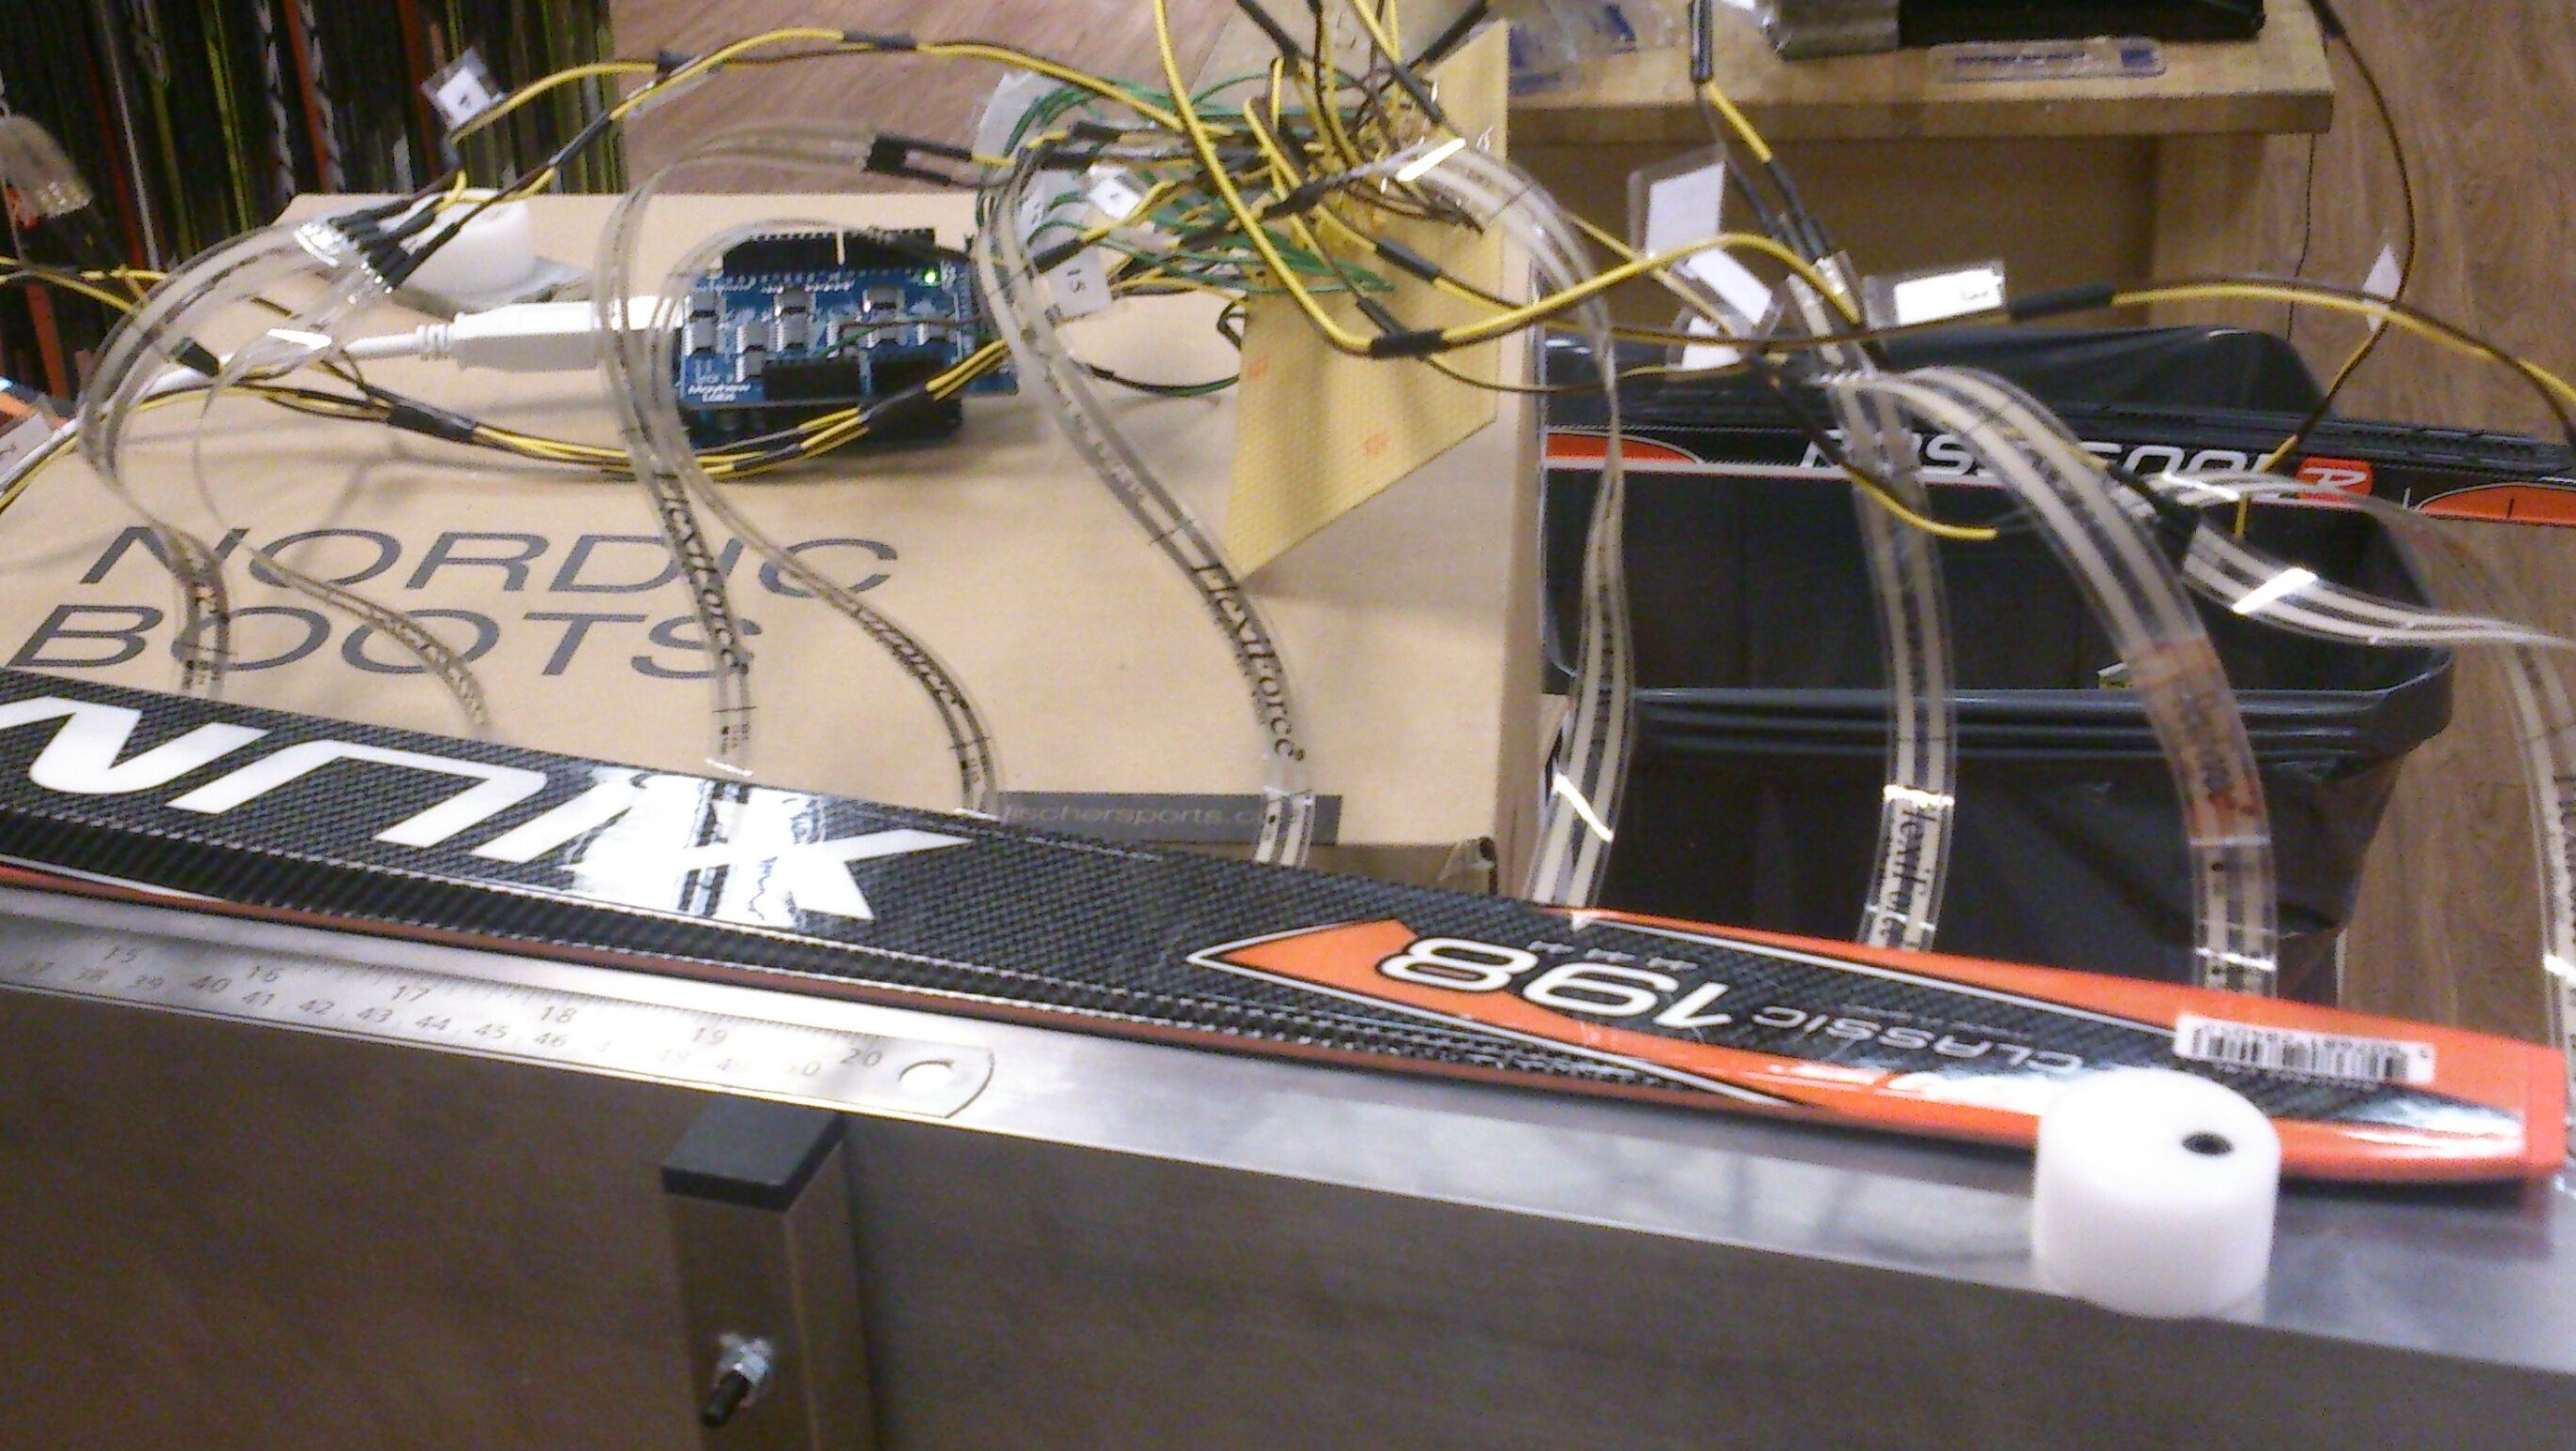
\includegraphics[scale=0.12]{figures/prototype2.jpeg}
    \caption{Photo of student research project led by Ole Marius Rindal and Jacob Norenberg}
    \label{fig:earlyprototype}
\end{figure*}

\begin{figure*}[!b]
    \centering
    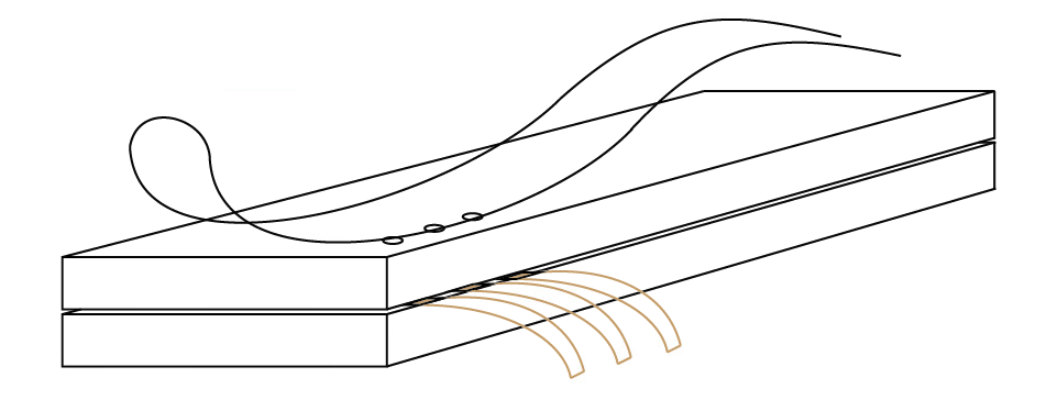
\includegraphics[scale=0.32]{figures/earlyconcept.png}
    \caption{Early concept on sensor placement and structure of a measurement device}
    \label{fig:earlyconcept}
\end{figure*}

To be able to apply force on vertically down on cross-country skis, and also for calibration of the sensors, one would need a digital weight press or manual weights placed on the BP. During the research done on possible ways of applying pressure, we were not able to find an easy solution. Reaching out to alternate resources was necessary.
After consulting with the Instrument Laboratory (I-Lab) at University of Oslo, Department of Physics, we came to a conclusion that the bottom surface had to be more rigid and withstand bending when applying force. I-Lab came up with a solution for applying forces on the ski linearly with a linear guide. This led to a 3D-modelled version of the sketch with the idea of using aluminum for the whole structure, giving the bench more stability and making it stiffer. The 3D-modelled sketch (Figure \ref{fig:3d-modelledsketch} and \ref{fig:3d-modelledsketch_front}) was drawn in AutoDesk Fusion 360 to visualize the concept of the test bench. It then became clear that to be able to produce such a test bench, one would need specialized computer numerical control (CNC) machine for accurate alignment of assembly points where the parts would need to be assembled. Further consultation with I-Lab, led to a collaboration where they were able to draw accurate models of the test bench and manufacture a test bench with the needed specifications for this thesis.
\begin{figure*}
    \centering
    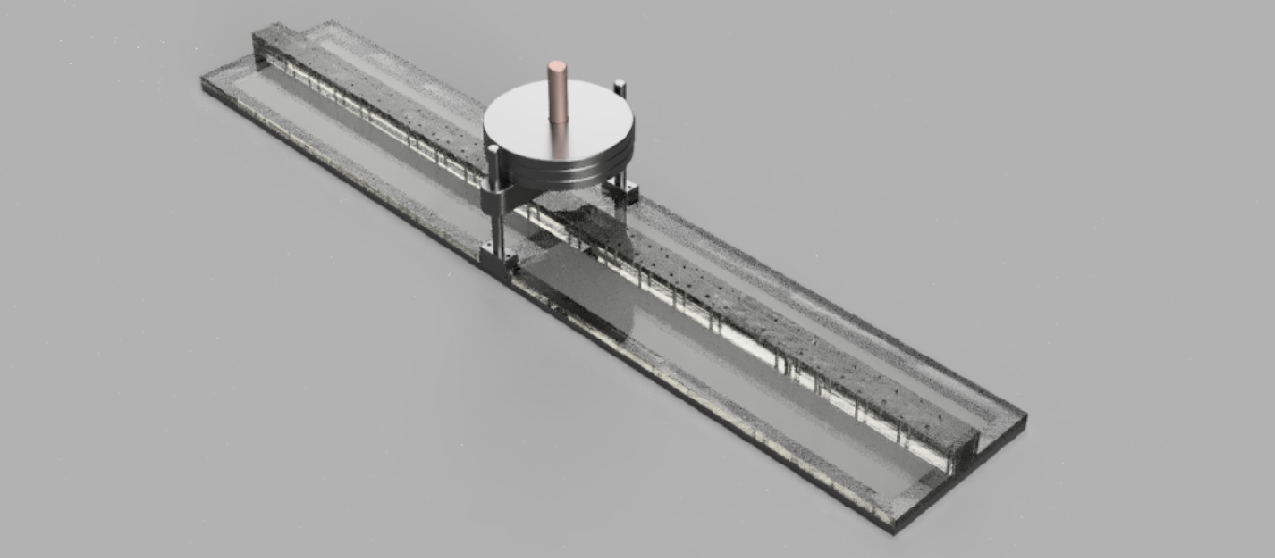
\includegraphics[scale=0.406]{figures/3dmodelledconcept.png}
    \caption{A 3D-model of the concept, drawn in AutoDesk Fusion 360 Student version}
    \label{fig:3d-modelledsketch}
\end{figure*}
\begin{figure*}
    \centering
    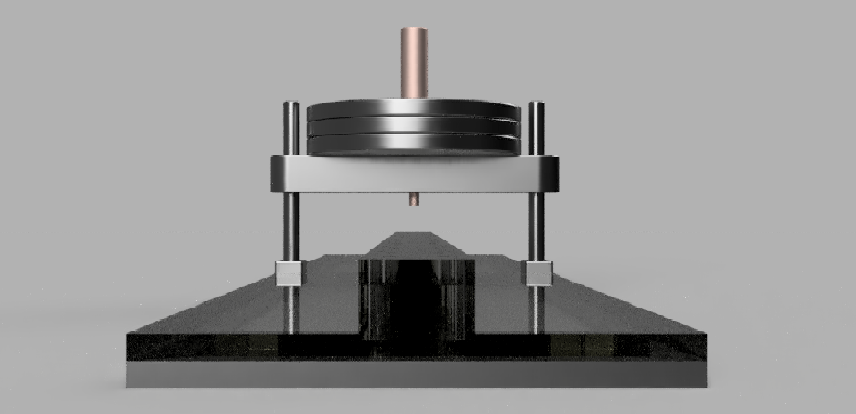
\includegraphics[scale=0.406]{figures/3dmodelledconcept_front.png}
    \caption{A 3D-model of the concept, drawn in AutoDesk Fusion 360 Student version, Front side}
    \label{fig:3d-modelledsketch_front}
\end{figure*}
For the sensors to be place accurately, small pockets were designed for a perfect fit of the sensors circumference. As Figure \ref{fig:3dpockets} show, the pocket holes guiding the sensor with an underlying "puck" (or piston) for a pinching effect on the sensor. This pinching effect was described to give more accurate results in measurements, using pucks on either side of the sensor \citep{vecchi_experimental_2000}. The "pucks" needed to cover at least $80\%$ of the measurement area on the sensor \citep{tekscanA201}. The pockets were placed with a center-to-center distance of $25mm$ along the whole length of the measuring block of $215cm$ containing the sensors. And, with a second row with a center-to-center distance across of $30mm$. This was done for the flexibility of placing and moving the sensors to areas of interest, leaving the empty pockets unused. The linear weight guide was designed to load the weight linearly down on the BP of the ski. With the additional option of a adjustable plate, representing of a foot to adjust the loading point offset from the BP. This was designed with the thought of being able to investigate pressure distribution characteristics at different ski phases, being gliding-phase and kicking-phase.
A locking mechanism was placed at the back end of the measurement block, for the ski to be locked in place centered. This, in combination of the attached adjustable plate at the linear weight guide, would in theory center the ski perfectly on the measurement block. 
\begin{figure*}
    \centering
    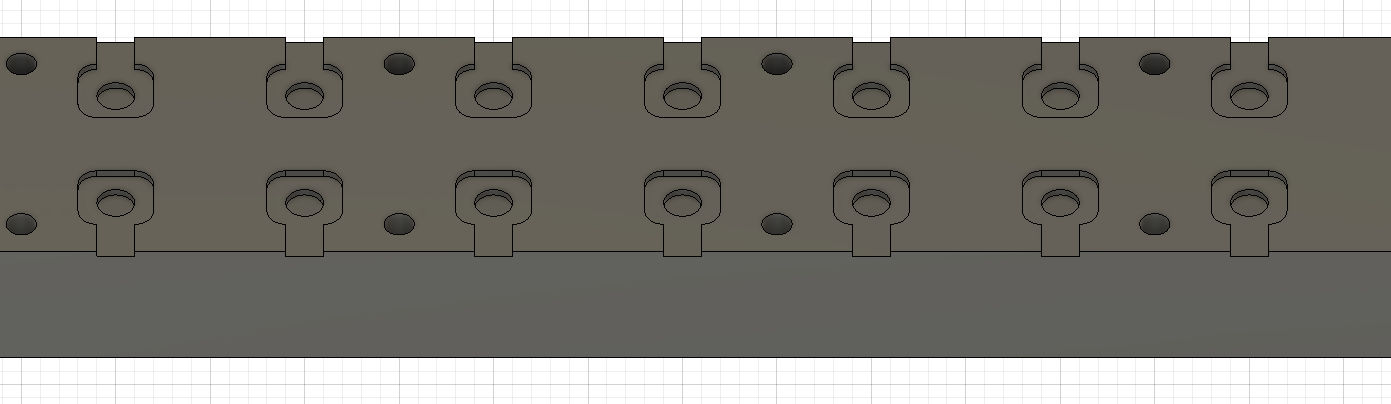
\includegraphics[scale=0.3]{figures/pockets.png}
    \caption{A 3D-model of the pockets for sensor placement}
    \label{fig:3dpockets}
\end{figure*}

The upper part of measurement block have holes of $9mm$ drilled out, for brass pistons or weight transfer pins (WTP) to be placed. As described earlier in this section, this would create a pinching effect on the sensor with the bottom piston part in the pockets. These upper brass pistons of $8mm$, were designed with a detachable plastic cap with threading. These rounded plastic caps would be used for free movement of the ski on top of the WTP.

An additional tool was designed for proper calibration of the sensors. An aluminium beam attached placed on the center between two supporting legs which would rest on the test bench frame. At the end of the beam, a piston matching the hole size of the supporting guides on the measurement block was attached. Weights would then be placed on top of the beam, transferring the loaded weight on to the sensor when calibration of the sensor would be conducted (Section \ref{subsec:calibration}). 

\section{Sensors}
\label{sec:sensors}
\subsection{Pressure sensitive films}
Pressure-sensitive films are simple and thin sensors that are using to measure forces in areas where space is an issue or a requirement. Thin- or thick-films sensors like this can be seen in areas where one would need to register changes in forces to a solid or flexible surface. These force sensing sensors are also referred to as Force Sensing Resistors (FSR). Pressure sensitive films and force sensing resistors are sensors whose resistance decrease with increasing applied force.

\subsubsection{Construction of the sensor}
The name pressure-sensitive film sensor would seem to come from the way it is constructed. The sensor is typically based on five layers. As shown in Figure \ref{fig:sensorconstruction}, the five layers may be the two protective films, which envelopes the sensor as a protective layer. In between, we find the two electrodes enclosing the layer of ink. The electrodes allow electrons to flow through the ink from one electrode to the other.

\begin{figure*}[!b]
    \centering
    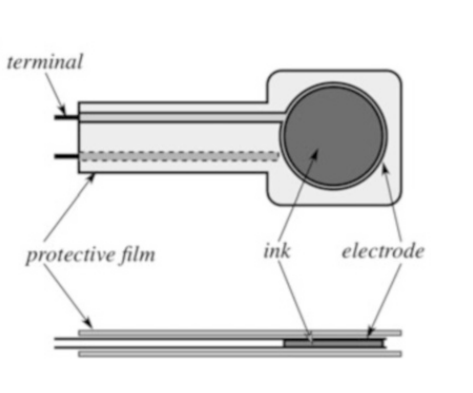
\includegraphics[scale=0.75]{figures/sensorconstruction.png}
    \caption{Composition of thin-film pressure sensor. Figure taken from \cite[p.418]{handbook}}
    \label{fig:sensorconstruction}
\end{figure*}

\subsubsection{Materials}
\label{subsec:materials}
The electrodes can be produced from any conductive material. In terms of producing cheap and reliable sensors, materials like silver can be used. Film materials used as protective layer should be elastic and flexible to allow movement when applying force on the sensor. Flexible material like dielectric Polyester can be used, which also insulates the electrodes. The ink used to conduct electrons between the electrode plates is described to be produced by screen printing piezoresistive ink with a predefined pattern. The ink is printed as thick films having a thickness ranging from 10$\mu m$ to 40$\mu m$. The ink is later dried at 150\textdegree C and then sintered from 700\textdegree C to 900\textdegree C. The sintering makes grains of conductive and insulating oxides bind together and give them cohesion and strength. This results in the ink containing small submicron particles of various metal oxides \citep[10.3, p.418]{handbook}.

\subsubsection{How does the sensor register force?}
When applying force to the sensor, the conductivity increases by increasing connection between the electrodes through three main mechanisms.
The three different mechanisms are conduction, hopping and tunneling.
Based on these, the amount of electrons passing through the ink, increases with more force on the sensor. As shown in Figure \ref{fig:sensorconcept}, conduction is direct contact in the particles of the ink, this happens when the particles are fully connected. Hopping happens when the particles are close enough to allow the electrons to jump. Typically, the jumping effect happens when the distance between the particles are around 10$nm$. The final mechanism is tunneling. This happens when the particles are barely touching (at around 1$nm$) and establishes a path for the electrons \citep[10.3, p.418]{handbook}.

\begin{figure*}[!b]
    \centering
    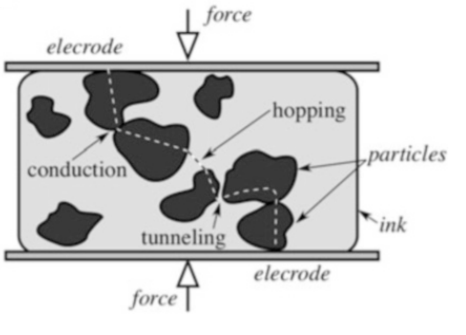
\includegraphics[scale=0.75]{figures/sensorconcept.png}
    \caption{Concept of pressure-sensitive ink. Figure taken from \cite[p.418]{handbook}}
    \label{fig:sensorconcept}
\end{figure*}

\subsubsection{Usage}
The sensor operates in the voltage area of the input voltage of the circuit. This can typically be from $0V$ to $+5V$. By applying force on the sensor, the resistance decreases and conductivity increases. This allows the output voltage to vary, which allows for a simple way of reading and measuring. When the sensor is idle, without load, the sensor is described to have mega-ohms of resistance or infinite impedance. This makes the idle state difficult as a minimum value for calibration. The sensor should be loaded with a small weight, covering around 80\% of the sensor's measuring surface \citep[10.3, p.418]{handbook}. Due to potential noise and spikes in the measurement, one should consider low-pass filtering with a capacitor, this is later tested in Chapter \ref{subsec:capacitor}.
The circuits used are simple voltage dividers or operational amplifier circuits. Where the latter prevents the sensor to draw power directly from the supply voltage. For best results, one should consider different circuits for specific application area.

\subsubsection{Measurement quality}
The pressure-sensitive sensor is known for having linear measurements (the linearity error can typically be $\pm$ 3\%) and has a moderate application difficulty. The measurements do on the other hand have some issues when it comes to measuring over longer periods of time. The ink material need time to reset after a period of measuring. The conductance can increase exponentially and the data is no longer useful. The measurements tend towards non-linear.
Allowing of the ink to settle to ensure consistency in the results is something that is considered when gathering data \citep{vecchi_experimental_2000}.

\subsection{FlexiForce A201 Sensor}
\label{subsec:flexiforce}
The FlexiForce A201 sensor from Tekscan is a pressure sensitive film, constructed of two layers of plastic substrates films like polyester. Each layer consists of a conductive material (silver), which encloses a layer of conductive ink with adhesive, as described in Section \ref{subsec:materials}. The sensing area is defined by a circular pattern of $10mm$, extended to two connectors for reading voltage (Figure \ref{fig:tekscana201}. Tekscan, Inc. offers three variations of the FlexiForce A201 sensor. Low$^1$ 4,4\si{\newton}, Medium$^2$ 111\si{\newton}, and High$^3$ 445\si{\newton}, where the latter can be adjusted to have a sensing area up to 4448\si{\newton} by adjusting the sensitivity in the circuit \citep{tekscanA201}. The idle state of the flexiforce A201, is described to have mega-ohms resistance, making it difficult to read accurate voltages when the sensor is not under load.
\begin{figure*}
    \centering
    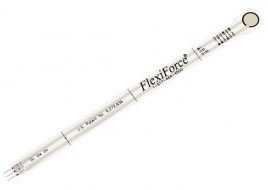
\includegraphics[scale=0.85]{figures/A201.jpg}
    \caption{Force sensing sensor (by Tekscan, Inc.). Figure taken from \textit{https://www.tekscan.com/products-solutions/force-sensors/a201}}
    \label{fig:tekscana201}
\end{figure*}

\subsection{Interlink Force Sensing Resistor}
\label{subsec:interlink}
The Force Sensing Resistor (FSR) from Interlink Electronics is a common device used for sensing changes in force from contact, with an optimized sensitivity for use human touch \citep{interlinkelectronics}. The FSR sensor is a thick-filmed sensor consisting of two conductive layers with interdigitated patterns which is commonly found in heat sensors. The interdigitated layers are deposited on a thermoplastic sheet facing another sheet containing a conductive polyetherimide film. A spacer placed between the sheets allows electrical contact when force is applied \citep{vecchi_experimental_2000}. As the FlexiForce A201 sensor, it is based on a circular construction with a diameter of $14.7 mm$ (Figure \ref{fig:fsr402}). 

\begin{figure*}
    \centering
    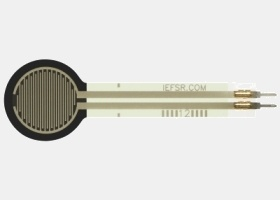
\includegraphics[scale=0.85]{figures/FSR-402.jpg}
    \caption{Force sensing resistor (FSR by Interlink Electronics). Figure taken from \textit{https://www.interlinkelectronics.com/fsr-402}}
    \label{fig:fsr402}
\end{figure*}

\subsection{Calibration of the sensors}
\label{subsec:calibration}
The calibration of the sensor can be done by calibrating the sensor at a minimum- and maximum-weight. Followed by a line fit to create the system response. This works well if we know the linearity of the measurements. If the conductance versus force linearity is known to increase more exponentially, we should consider using knots to section out certain parts of the full scale output. If the measurements should result in non-linearity's, the sensor could be damaged.

\section{Circuits}
\label{sec:circuits}
For measuring the response of a pressure-sensitive film, a circuit should be formed to obtain stable and accurate measurements. Since a sensor draws power from the circuits power source, one will see current drops when applying pressure to the sensor in a regular RC (Resistor-Capacitor) circuit or in a voltage divider. This is where a operational amplifier circuit will come to great benefit.

\subsection{Voltage divider}
A voltage divider is one of the simplest forms of circuits (Figure \ref{fig:voltagedivider}) considered for a pressure-sensitive film. The quality of the measurement result is based on the voltage read from the circuit. The voltage varies when the resistance of the sensor changes due to applied pressure. This voltage is based on the analytic formula in Equation \ref{eq:voltagedivider}. 
\begin{equation}
\label{eq:voltagedivider}
    V_{out} = V_{supply} \cdot \frac{R_1}{R_{flexiforce} + R_1}
\end{equation}
\begin{figure*}[!b]
    \centering
    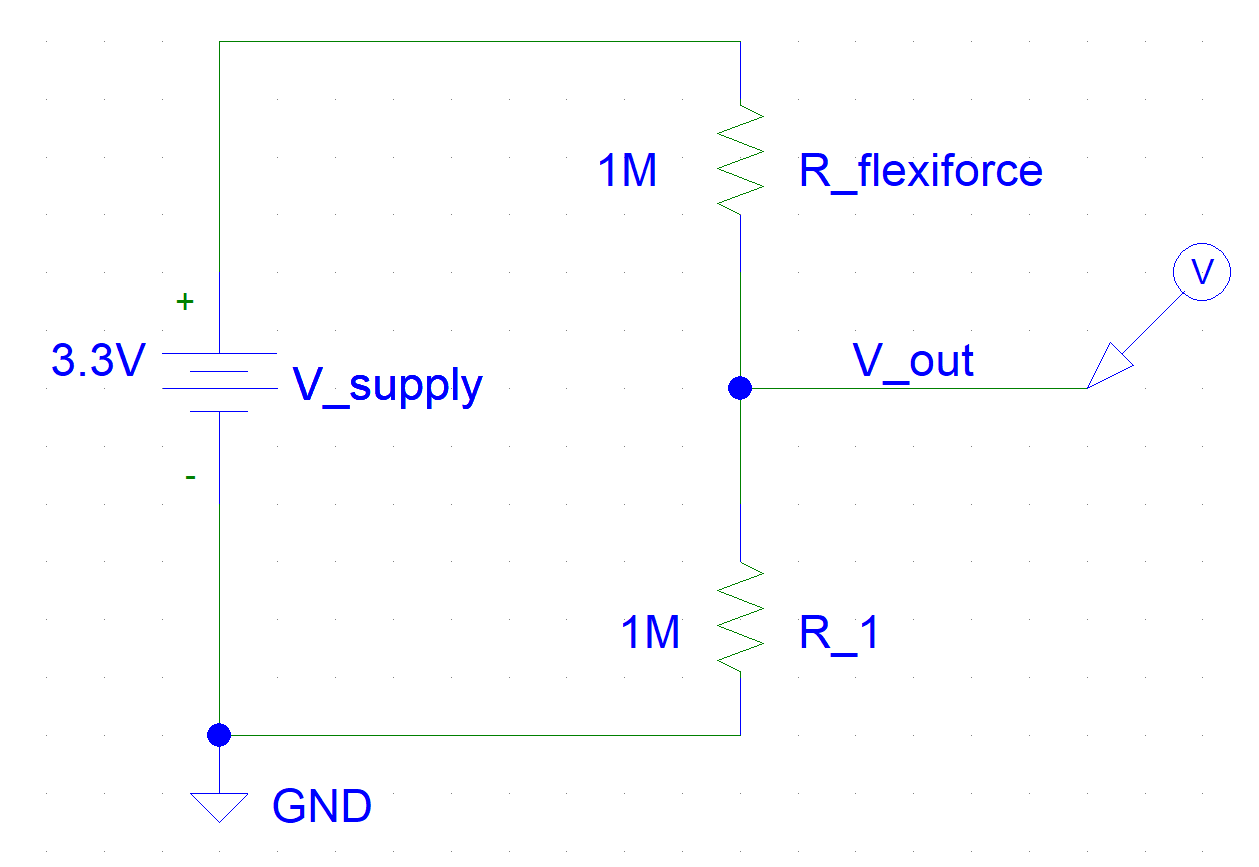
\includegraphics[scale=0.45]{figures/voltage_divider.png}
    \caption{Voltage divider circuit for sensing changes in pressure sensitive films}
    \label{fig:voltagedivider}
\end{figure*}
When applying pressure on the sensor, the resistance decreases, resulting in an increase in voltage in $V_{out}$. This voltage can be calibrated and transformed directly to weight ($Kg$) for the specific sensor in use. One of the benefits of using a voltage divider, is the easy implementation. On the contrary, we can experience more interference in the measured voltage and measurement spike due to the sensor drawing power straight from the power source. !Kg formula

\subsection{Operational amplifier circuits}
\label{subsec:opamps}
Operational amplifiers are 3 terminal devices used to amplify voltages, two inputs and 1-output, with an addition of power connections ($V_{supply}$). These so called OP-amps are described to have infinite input impedance, meaning it has infinite resistance on the two inputs, making current impossible to flow between them. And, zero output impedance. This is the case for ideal Op-amps, where in the real world applications, no Op-amp is perfect and some variations in current and voltage may occur. Operational amplifiers can be connected into two main forms of circuits, the \textit{Inverting operational amplifier circuit} and \textit{Non-inverting operational amplifier circuit}. By leaving the two inputs open, the ideal operational amplifier is defined to be in a "Open-loop"-state, resulting in infinite gain (A) and bandwidth. In real world applications, the gain can be adjusted by increasing or decreasing the feedback- or input-resistance and is a measure of how good a operational amplifier is. The power connectors on the operational amplifier is defined as $V_{supply}$, which decides the operational voltage range of the amplifier. This operational voltage range usually caps at $\pm 15V$, which gives us a upper limit of how much the circuit is able to amplify a signal.

\subsubsection{Inverting Operational amplifier circuit}
The inverting operational amplifier (Figure \ref{fig:invertingopamp}) is based on the characteristics described in Section \ref{subsec:opamps}. It is the version of the Op-amp circuit that connects the feedback to the negative input (negative feedback) of the two available, making the state of the op-amp "closed-loop". This results in an amplified signal with a negative sign, giving an overall reduced amplification. In this case, the pressure sensitive film, is connected as the $R_{in}$ resistor, which allows the output voltage $V_{out}$ to vary from $0V$ to $-V_{supply}$. When applying force to the sensor, resistance decreases and voltage on the output increases (Equation \ref{eq:invopamp_amplifier_vout}).

\begin{equation}
\label{eq:invopamp_amplifier}
    A = \frac{V_{out}}{V_{in}} = - \frac{R_{feedback}}{R_{flexiforce}}
\end{equation}

\begin{equation}
\label{eq:invopamp_amplifier_vout}
    V_{out}= -V_{in} \cdot \frac{R_{feedback}}{R_{flexiforce}}
\end{equation}

\begin{figure*}
    \centering
    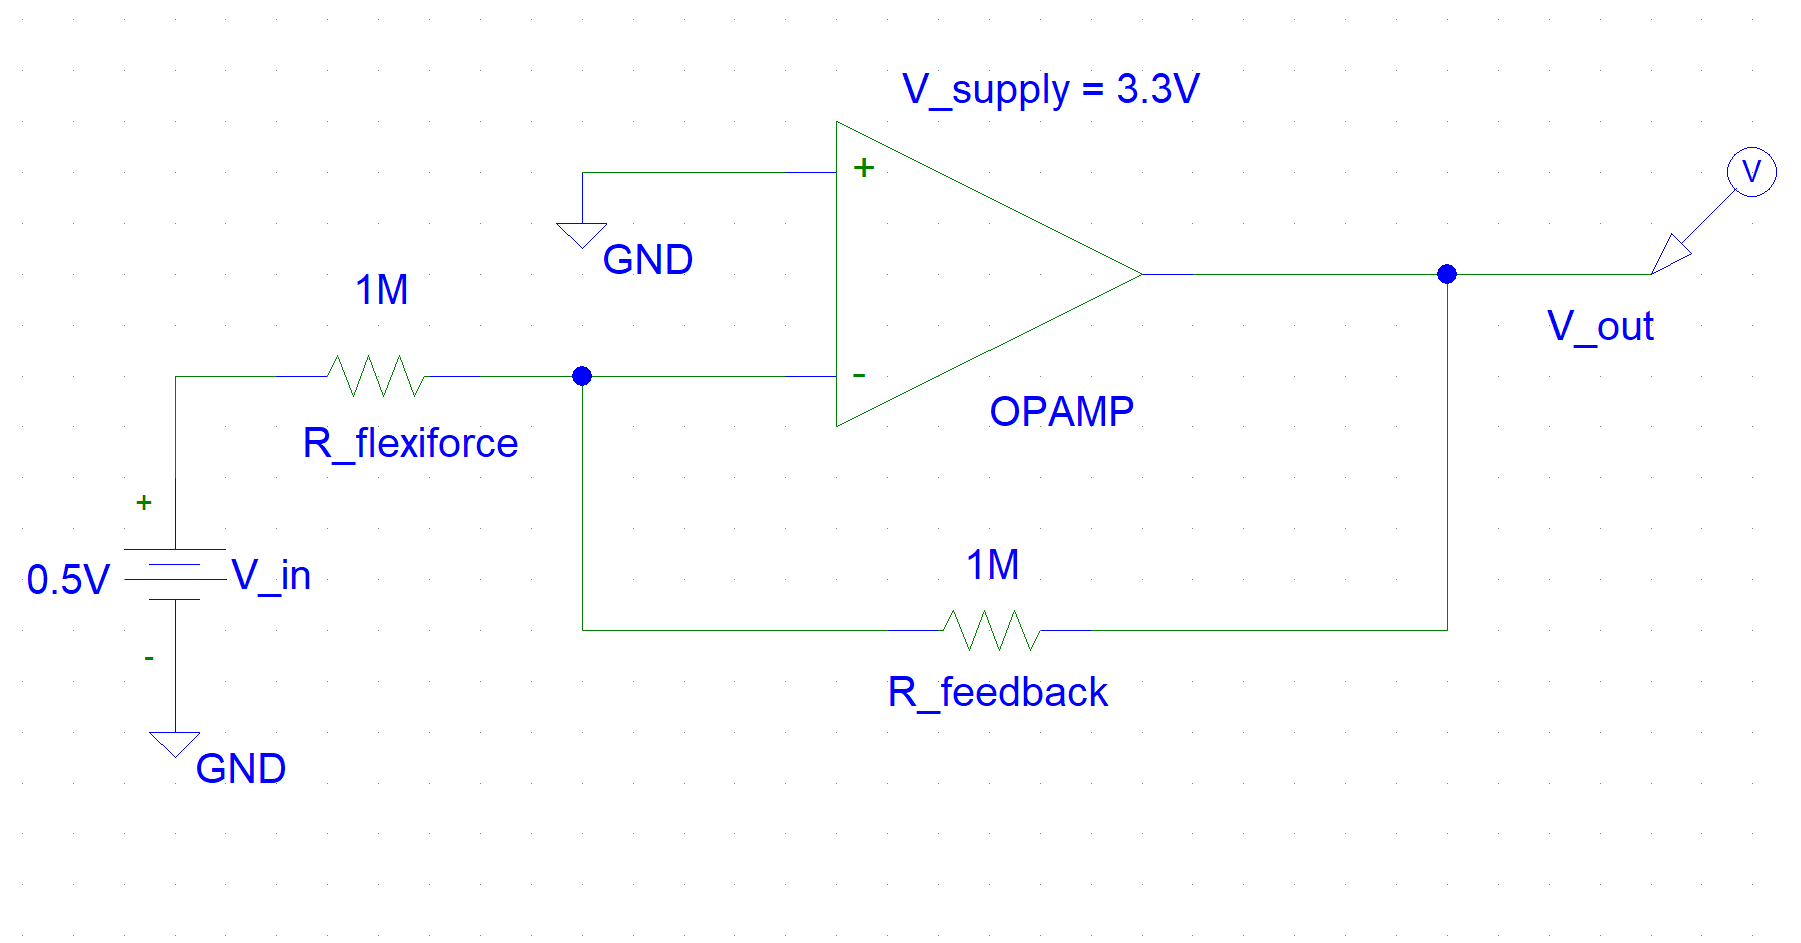
\includegraphics[scale=0.3]{figures/inverting_opamp.png}
    \caption{Inverting operational amplifier circuit for sensing changes in pressure sensitive films (in unity state A=1)}
    \label{fig:invertingopamp}
\end{figure*}


\subsubsection{Non-inverting operational amplifier circuit}
Much like the Inverting operational amplifier, the non-inverting version (positive feedback) connects its feedback to the negative input on the op-amp, but is running voltage input on the positive side. With the addition of feedback running to ground (Figure \ref{fig:noninvertingopamp}). The effect of using a non-inverting operational amplifier circuit is an overall increase in gain compared to the inverting op-amp circuit. Due to the overall increase in amplification, seen from Equation \ref{eq:noninvopamp_amplifier_vout}, one can experience instabilities in the output for lower values of voltage (micro volts).
\begin{equation}
\label{eq:noninvopamp_amplifier}
    A = \frac{V_{out}}{V_{in}} = 1 + \frac{R_{feedback}}{R_{flexiforce}}
\end{equation}

\begin{equation}
\label{eq:noninvopamp_amplifier_vout}
    V_{out} = V_{in}(1 + \frac{R_{feedback}}{R_{flexiforce}})
\end{equation}

\begin{figure*}
    \centering
    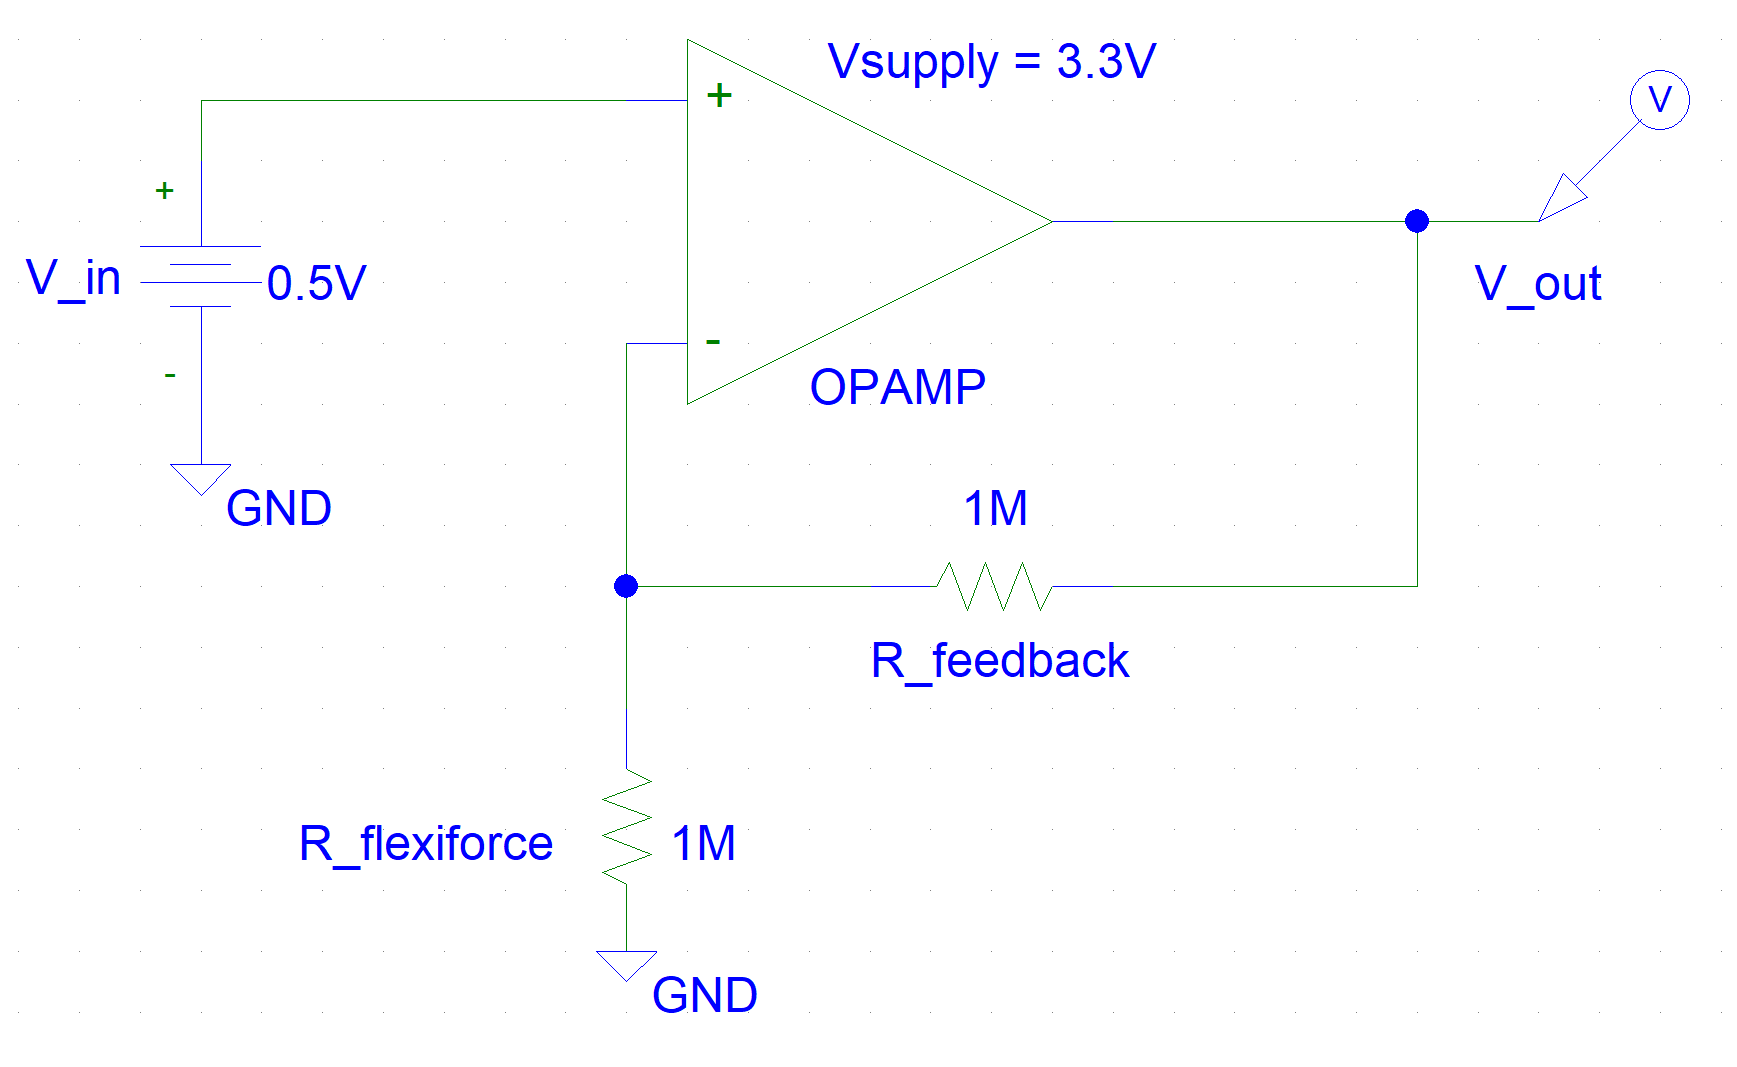
\includegraphics[scale=0.3]{figures/noninverting_opamp.png}
    \caption{Non-inverting operational amplifier circuit for sensing changes in pressure sensitive films}
    \label{fig:noninvertingopamp}
\end{figure*}

\subsection{Implementation of a capacitors}
\label{subsec:capacitor}
When it comes to implementing a analog low-pass filter, a capacitor in parallel with the feedback resistance is implemented in the operational amplifier circuits (Figure \ref{fig:capacitor}) as a first order low-pass filter. One would see this as an option to deal with high frequency spikes in the measurements. The capacitors function in parallel with a resistor, is to filter out higher frequencies, dependent on the size of the capacitor. When the capacitor reaches its cutoff frequency $\omega$, it causes a short in the circuit, leading all frequencies higher than the cutoff frequency to ground or a specified point in the circuit. A larger capacitor will have lower higher cutoff frequency as defined in Equation \ref{eq:cutoff}. By introducing the capacitor, it causes an extra pole in the frequency response of the amplifier circuit, making it more stable. Additionally, introducing capacitors by the power supply and the output of the circuit, additional means of fighting noise in the circuit is introduced.

\begin{equation}
\label{eq:cutoff}
    \omega = \frac{1}{R_{feedback}C_1}
\end{equation}

\begin{figure*}
    \centering
    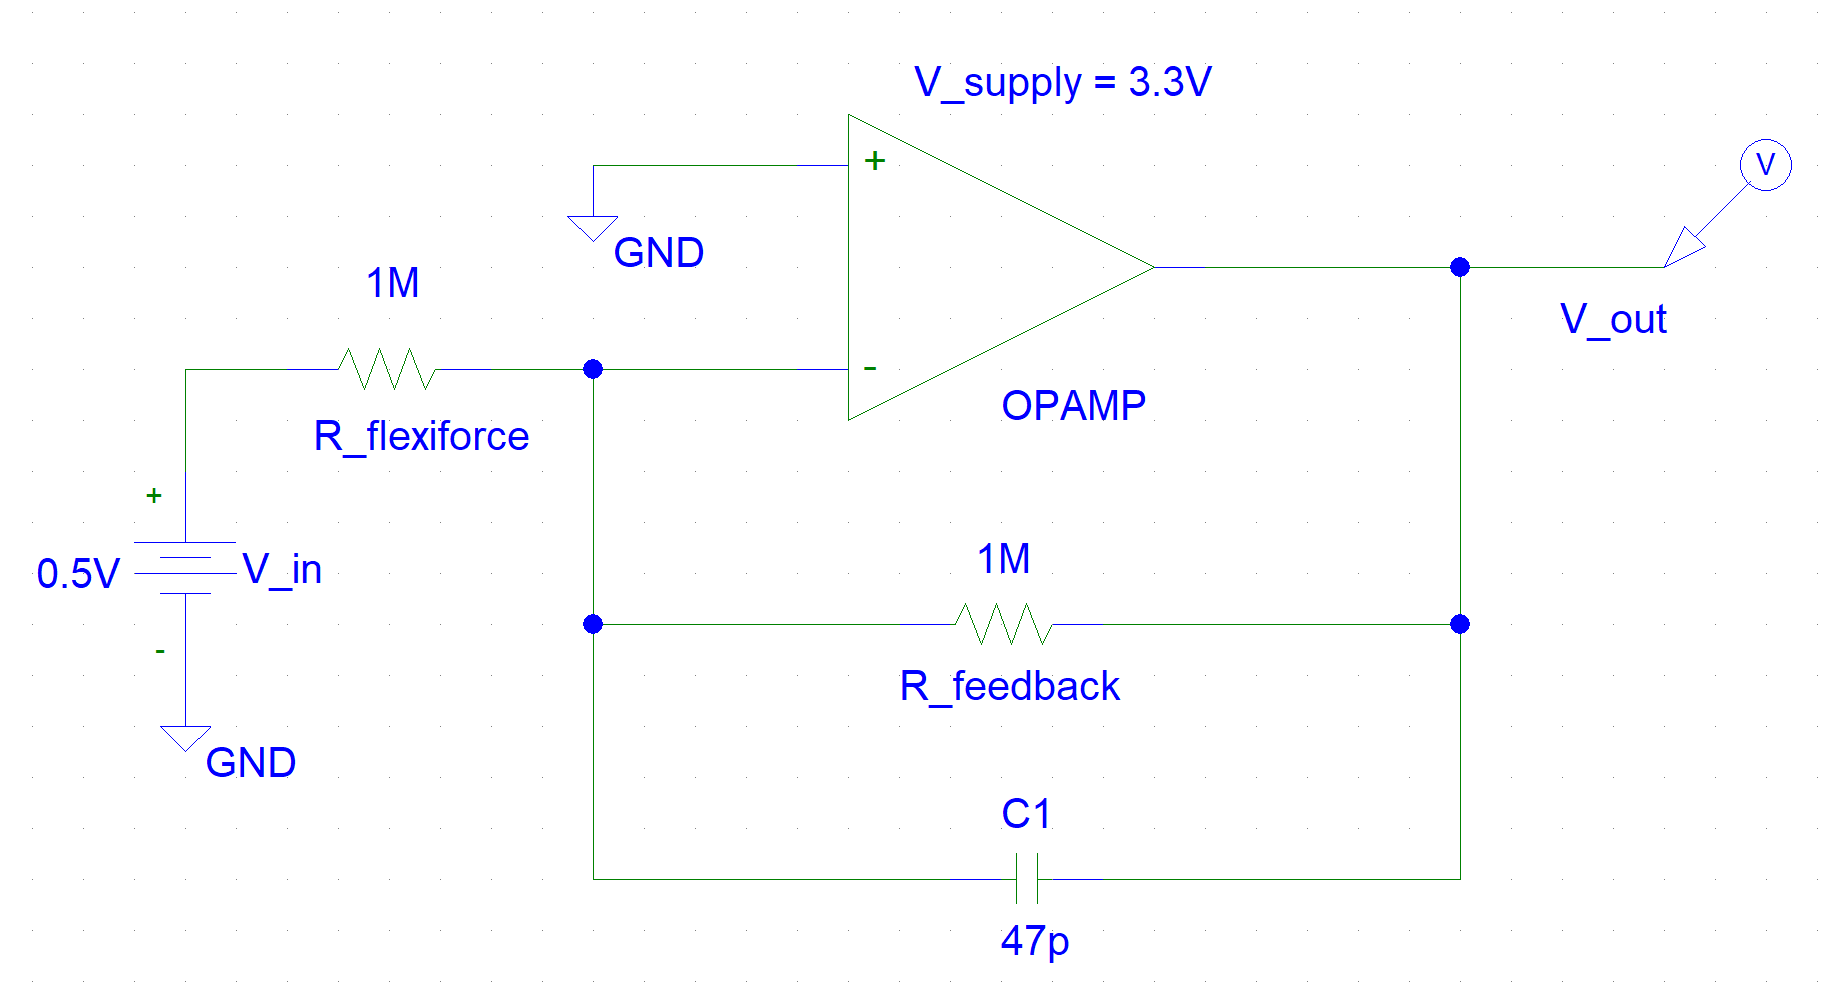
\includegraphics[scale=0.28]{figures/capacitor.png}
    \caption{Inverting operational amplifier circuit with capacitor}
    \label{fig:capacitor}
\end{figure*}


\section{Calibration methods}
Calibration is an essential part of a measurement process and should be done regularly for consistent results. This section explains the concept of calibration why we do it.

\subsection{Modifying the full scale output}
The full scale output (FS) is the relation between input stimulus ($s$) and the output response. It defines the maximum value the system is able to output with given stimulus. Essentially, the full scale output is the measured voltage from the measurement system and can be modified digitally when reading the voltage.
The calibration method can typically be to create a system response based on a statistical line fitting model between a minimum- and maximum-value. For calibration in this thesis, we will see calibration be done with weights in five stages with different weights (also known as calibration knots). This is done by telling the system what weight has been loaded and referring this to the amount of voltage read by the micro controller (Chapter \ref{chap:microcontrollers}).

\subsection{Calibration weights}
For the sensors to be calibrated correctly, we are required to have a absolute scale of weights to refer our voltages to. This can be a certain amount of weights increasing linearly to the appropriate application area. For this thesis, a absolute scale can for example be from 1\si{\kilogram} to 20\si{\kilogram}. 

\section{Chapter results}
\label{sec:chapresults3}
Discussing the results gathered when finding the correct circuit with flexiforce, and calibration results.

\section{Chapter discussion}
In the process of selecting a force sensing sensor, it is required to chose the most suited sensor for the application area. In the research done by Fabrizio Vecchi and his colleagues \citep{vecchi_experimental_2000} on commercial sensors in biomechanics and motorcontrol, sensors like the \textit{Flexiforce A201 \ref{subsec:flexiforce}} and \textit{Force Sensing Resistor \ref{subsec:interlink}} were evaluated. In terms of linearity, time-drift tests and robustness, the Flexiforce sensor presented better results. As mentioned, the application area is what determines the choice of sensor, and for this thesis a sensor is required for handling forces significantly higher than previous research. The Flexiforce sensor in combination with the operational amplifier circuits prove to show similar results in terms of linearity, which is a key factor to obtain consistent results in measurements.

\section{Chapter conclusion}
Sensors and circuits presented in Section \ref{sec:sensors} and \ref{sec:circuits}, the linearity and consistency of measurements were tested and evaluated. Differences were found in terms of noise (measurement spikes and variance), linearity and precision. An operational amplifier circuit was selected reasoned by the requirement of precise measurements and linearity. In combination with the Flexiforce A201 sensor, the system was able to handle the required forces up to 450\si{\newton} (or 45-46\si{\kilogram}). As suggested by Tekscan, Inc., a inverting operational amplifier circuit was chosen.
External and internal noise were handled by implementing a capacitor as a analog low pass filter, which proved to affect on the quality of the sampled data.
\begin{itemize}
    \item \textbf{!! How I calibrated and why}
\end{itemize}
